\section{Experiments}


Our experiments were intended to study SAMNet's performances as well as generalization abilities in different settings. For this purpose, we use two different versions of the COG dataset, an easy one (canonical) and a hard version to explore a wide range of difficulties. The following parameters control the difficulty level: the number of frames in the input sequence, the maximum memory duration (how far is the last object to be remembered), and the number of distractors. These parameters are detailed in Table 1 for each setting. The table also shows the size of the training/validation/test split used for our experiments. The COG dataset is composed of 44 tasks that have equal number of samples.
We chose to focus our effort only on the the 22 classification tasks.
We compare our model to the original COG model  ~\cite{yang2018dataset} using their implementation (https://github.com/google/cog) and scores given by the authors. We also use the exact same training parameters detailed in the original paper.

On the other side we trained SAMNet using IBM's Mi-Prometheus~\cite{kornuta2018accelerating}, a framework for research based on Pytorch. We trained all our models using NVIDIA’s GeForce GTX TITAN X GPUs. We trained  SAMNet using 8 reasoning steps SAMCells and a hidden state size of 128. The external memory has 128-bit slots. We trained our model until convergence but we also have set a training time limit of 80 hours.



\begin{table}[!t]
	\centering
	\caption{COG Dataset parameters for the canonical setting and the hard setting  }
	\begin{tabular}{ccc}
		\toprule
		Dataset       &    Canonical setting   & Hard setting   \\
		
		\midrule
		
		number of frames      &    4  &  8      \\
		
		\midrule
		
		maximum memory duration      &    3   & 7      \\
		
		\midrule
		
		number of distractors     &    1   & 10    \\
		
		\midrule
		
		size of training set    &    10000320  & 10000320      \\
		
		\midrule
		
		size of validation/test set    &    500016   & 500016      \\
		
		\midrule
		
		tasks per family  training set   &    227280  & 227280    \\
		
		\midrule
		
		tasks per family  validation/test set   &    11364   & 11364      \\
		
	
	
		
	
	   \bottomrule
	
	\end{tabular}
	
	\label{tab:parameters}
\end{table}


\subsection{Training and testing Methodology}

First we evaluate SAMNet's performance on the canonical setting and compare it with the COG Model. As shown in Table 2 we could achieve a small improvement in accuracy, from 97.6\% for the COG model to 98\% for SAMNet.

Our second goal is to improve the accuracy on the hard dataset. In order to do this, we have tried three different approaches.

The first approach is to train a model on the hard training set only and test it on the hard test set. It is the same approach used by the original COG paper ~\cite{yang2018dataset} to evaluate performance on the hard dataset. We achieve a test accuracy of 91.9 \% which represents a 12\% improvement from the COG model score (see Table 2).
It shows that SAMNet's design choices make a difference when it come to harder tasks with longer sequences and more distractors objects.

The second approach is to see if we can generalize from the easy to the hard setting. We train a model on the canonical dataset and test it on the hard dataset. Doing so we can achieve comparable results than the first approach. It shows that SAMNet has good generalizations abilities. It can adapt well to different sequence lengths and number of distractors.

Finally we train a model on the canonical data set, fine-tune it on the hard data set during only 25k iterations and test it on the hard dataset. Thanks to fine-tuning, we can observe a significant improvement from 91.6\%  to 96.5\% test accuracy which represents the state of the art accuracy for the hard setting (classification tasks).
After a short fine-tuning process, the model can generalize well to harder tasks and even surpass the accuracy obtained in the first approach. We note that the third approach is two time faster than the first one and more effective.


We can also notice a major improvement for the two hardest tasks, AndCompareShape and AndCompareColor. Those two tasks represent a higher level of difficulty due to the number of objects to be remembered in order to answer the question correctly.
As we can see in Table 2 we could achieve a 12\% improvement for the canonical data set and almost a 40\% improvement for the hard dataset.
We see that the SAMNet's external memory plays an important role in remembering objects from the past and this affects the test scores significantly. 






\begin{table}[t]
	\tiny
	
	\caption{COG test set accuracies for  SAMNet \& COG models. For the COG section, the results marked as 'paper' comes from the original COG paper ~\cite{yang2018dataset}, whereas the results marked as 'ours' come from our own experiments using the following implementation: https://github.com/google/cog }
	
	\centering
	\begin{tabular}{ccccccccccc}
		\toprule
		Model & & SAMNet & && && COG&& \\
		\cmidrule{2-5} \cmidrule{7-11} 
		&&&&& & paper & ours & ours & paper&\\
		\cmidrule{7-9} \cmidrule{10-11}
		Trained on       & canonical & canonical & canonical & hard &           &  canonical  & canonical  & canonical & hard \\ 
		Fine tuned on  & - & - & hard  & - &           & -   & - & hard & - \\ 
		Tested on        & canonical & hard & hard & hard &            &canonical  & hard & hard & hard  \\ 
		\midrule
		
		Overall accuracy & 98.0 & 91.6 & 96.5  & running &           & 97.6  & 65.9 & running& 80.1 \\ 
		
		\midrule 
		
		
		AndCompareColor	&	93.5		&	82.7	&	89.2	&&		&81.9	&53.1&&	51.4
\\ 
		AndCompareShape	&	93.2 		&	83.7	&	89.7	&&	&	80.0	&57.1	&&50.7\\ 
		AndSimpleCompareColor	&	99.2	&		85.3	&	97.6	&	&	&99.7&	53.4&&	78.2\\ 
		AndSimpleCompareShape	&	99.2&			85.8	&	97.6	&&	&	100.0	&56.7&&	77.9\\ 
		CompareColor	&	98.1		&	89.3	&	95.9	&&		&99.2&	56.1&&	50.1\\ 
		CompareShape	&	98.0	&		89.7	&	95.9	&&	&99.4	&66.8	&&50.5
\\ 
		Exist	&	100.0	&		99.7	&	99.8		&&	&	100.0&	63.5&&	99.3\\ 
		ExistColor	&	100.0		&	99.6	&	99.9	&&	&	99.0&	70.9&&	89.8\\ 
		ExistColorOf	&	99.9	&		95.5	&	99.7		& & &	99.7&	51.5&&	73.1\\ 
		ExistColorSpace	&94.1		&	88.8	&	91.0	&& &	98.9	&72.8	&&89.2\\ 
		ExistLastColorSameShape	&	99.5		&	99.4	&99.4	&&		&100.0	&65.0&&	50.4
\\ 
		ExistLastObjectSameObject	&	97.3	&		97.5	&	97.7	&&	&	98.0&	77.5	&&60.2\\ 
		ExistLastShapeSameColor	&	98.2		&	98.5&	98.8	&&	&	100.0&	87.8&&	50.3\\ 
		ExistShape	&	100.0	&	99.5	&	100.0	&&&	100.0&	77.1	&&92.5\\ 
		ExistShapeOf	&	99.4		&	95.9	&	99.2	&&&100.0	&52.7&&89.8\\ 
		ExistSpace	&	95.3	&	89.7	&	93.2	&&		&	98.9	&71.1	&&92.8\\ 
		GetColor	&	100.0		&	95.8&	99.9	&& &	100.0&	71.4&&	97.9\\ 
		GetColorSpace	&	98.0		&	90.0	&	95.0&	& &	98.2	&71.8&&	92.3\\ 
		GetShape	&	100.0		&	97.3&	99.9&	&	&	100.0  &83.5&&	97.1
\\ 
		GetShapeSpace	&	97.5	&	89.4	&	93.9	&&&	98.1  &78.7	&&	90.3\\ 
		SimpleCompareShape	&	99.9		&	91.4	&	99.7	&	&&	100.0 & 67.7&&	99.3\\ 
		SimpleCompareColor	&	100.0 		&	91.6  &	99.80&	&	&	100.0&	64.2&&	99.3	  \\ 
		
		
		
		
		
		
		
		\bottomrule
	\end{tabular}
	\label{results}
\end{table}


\begin{figure}
	\centering
	\caption{Comparison of SAMNet and COG on their abilities to generalize from the canonical to the hard dataset. We show three different settings: 1) (baseline) trained on canonical, tested on canonical 2) trained on canonical, tested on hard, 3) trained on canonical, fine tuned on hard, tested on hard. }
	
	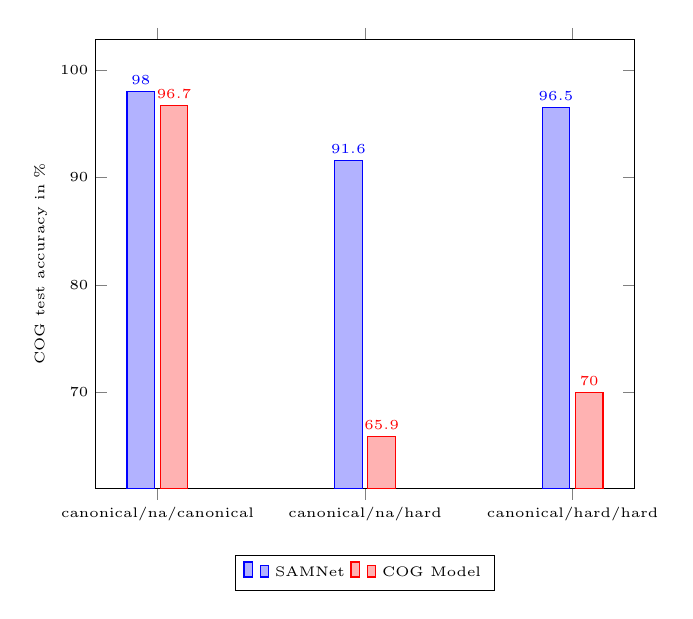
\begin{tikzpicture}
	
	
	
	\tiny
	
	\begin{axis}[
	ybar,
	enlargelimits=0.15,
	legend style={at={(0.5,-0.15)},
		anchor=north,legend columns=-1},
	ylabel={COG test accuracy in \% },
	symbolic x coords={canonical/na/canonical, canonical/na/hard, canonical/hard/hard},
	xtick=data,
	nodes near coords,
	nodes near coords align={vertical},
	]
	\addplot coordinates {(canonical/na/canonical,98) (canonical/na/hard,91.6) (canonical/hard/hard,96.5)};
	\addplot coordinates {(canonical/na/canonical,96.7) (canonical/na/hard,65.9) (canonical/hard/hard,70)};
	\legend{SAMNet ,COG Model}
	\end{axis}
	\end{tikzpicture}
\end{figure}


